
\chapter{Proof-of-work}

Het loterijsysteem dat in het vorige hoofdstuk is besproken, kent twee grote problemen:

\begin{enumerate}
    \item Als we ervan uitgaan dat we geen enkele centrale instantie kunnen vertrouwen, wie verkoopt dan de loterijloten en wie trekt de winnende nummers?
    \item Hoe kunnen we garanderen dat de loterijwinnaar de rest niet misleidt en enkel geldige transacties in het grootboek opneemt?
\end{enumerate}

Als we een systeem willen waar iedereen \textit{zonder toestemming} lid van kan worden, dan moeten we de eis dat iets betrouwbaar moet zijn uit het systeem halen; het systeem moet \textit{trustless} zijn.\footnote{Nvdr. vrij vertaald: \textit{zonder vertrouwen}. \textit{Trustless} houdt in dit geval in dat de gebruiker het systeem niet hoeft te vertrouwen, maar alles zelf objectief kan verifiëren.} 

Bij het ontwerpen van ons systeem moeten we de volgende factoren in aanmerking nemen:

\begin{enumerate}
    \item Bij gecentraliseerde loterijen, zoals de Staatsloterij, draagt één organisatie de verantwoordelijkheid voor het genereren van alle loten. In ons systeem is echter geen plaats voor een centrale autoriteit die we kunnen vertrouwen, dus moet iedere deelnemer in staat zijn om zelf zijn loten te genereren.
    \item  	We moeten erop toezien dat niemand volledige controle over de loterij krijgt door een overweldigend aantal loten te genereren. Daarom kunnen de loten niet gratis zijn. Maar hoe zorgen we ervoor dat je daadwerkelijk geld moet uitgeven om loten te kopen, als er niemand is bij wie je ze kunt kopen? De loten moeten van het universum ``gekocht'' worden: je moet dus elektriciteit verbruiken om ze te genereren.
    \item  	Alle andere deelnemers moeten gemakkelijk kunnen verifiëren of je de loterij gewonnen hebt, simpelweg door je lotnummer te controleren. Bij de Staatsloterij bepaalt de trekkingsmachine van de Nederlandse Loterij welk lot de winnaar is. Dit is echter niet mogelijk binnen een gedecentraliseerd systeem In plaats daarvan laten we iedereen van tevoren overeenstemmen over een getallenreeks. Valt je lotnummer binnen het vooraf bepaalde bereik, dan win je. We gebruiken een cryptografische truc om dit te doen met behulp van een \textit{hash-functie}.
\end{enumerate}

\section[Een asymmetrische puzzel die veel energie vergt]{Een asymmetrische puzzel die veel energie vergt}

Het elegante antwoord op al deze drie vraagstukken is \textit{proof-of-work}.\footnote{ Proof-of-work betekent letterlijk \textit{bewijs van uitgevoerd werk/gedane arbeid}} Dit element van ons systeem werd al in 1993, lang voor de komst van bitcoin, uitgevonden. Het is waarschijnlijk het lastigst te doorgronden aspect van onze loterij, daarom zullen we dit in de volgende hoofdstukken uitgebreid behandelen.\footnote{\href{https://en.wikipedia.org/wiki/Proof-of-work\_system}{https://en.wikipedia.org/wiki/Proof-of-work\_system}} 

Zoals we eerder (in punt 2) hebben geconcludeerd, moet het een flinke investering zijn om loten te genereren. Anders zou het voor iedereen mogelijk zijn om zomaar een oneindig aantal loten in handen te krijgen. Wat is gegarandeerd kostbaar en komt niet van een centrale autoriteit?

Dit is waar de fysica van bitcoin om de hoek komt kijken: volgens de eerste wet van de thermodynamica kan energie niet worden gecreëerd of vernietigd. Er bestaat niet zoiets als een ``gratis lunch'' als het op energie aankomt. Elektriciteit is altijd kostbaar omdat je het moet kopen bij elektriciteitsleveranciers of je eigen energiecentrale moet bouwen. In beide gevallen is het verwerven van elektriciteit een dure aangelegenheid.

Het idee van proof-of-work is dat je deelneemt aan een willekeurig proces, vergelijkbaar met het gooien van een dobbelsteen. Maar in plaats van de gebruikelijke zes zijden, heeft onze dobbelsteen ongeveer evenveel zijden als er atomen zijn in het universum. Om deze dobbelsteen te rollen, en dus nummers te genereren, moet je computer berekeningen uitvoeren die stroom verbruiken.

Om de loterij te winnen, moet je een getal achterhalen dat wiskundig is afgeleid van de transacties die je in het grootboek wilt vastleggen, plus het getal dat je met de dobbelsteen hebt gegooid. Mogelijk moet je miljarden, triljoenen of zelfs quadriljoenen keren de dobbelsteen werpen om dit winnende getal te vinden, waarbij je duizenden euro's aan energie verbruikt. Aangezien dit proces willekeurig plaatsvindt, kan iedereen zijn eigen loterijnummers genereren, zonder tussenkomst van een centrale autoriteit. Het enige wat je hiervoor nodig hebt, is de lijst met transacties die je wilt vastleggen in het grootboek en een computer die in staat is een willekeurig getal te genereren. 

Hoewel het vinden van een winnend nummer wellicht duizenden dollars aan verbruikte energie heeft gekost, hoeven andere mensen in het netwerk slechts enkele eenvoudige controles uit te voeren om jouw werk te verifiëren.

\begin{enumerate}
    \item Is het door jou opgegeven getal kleiner dan het vooraf afgesproken bereik?
    \item Is het getal inderdaad wiskundig afgeleid van een correcte reeks transacties die je in het grootboek wilt opnemen?
    \item Voldoen de voorgelegde transacties aan de regels van bitcoin (zijn er geen dubbele uitgaven, worden er geen nieuwe bitcoins gegenereerd buiten het toegestane schema, etc.)?
\end{enumerate}

Het proces van 'proof-of-work' is gebaseerd op toeval en vereist talloze computerbewerkingen om een winnend lot te vinden. Het controleren ervan vergt echter slechts een enkele handeling. Je zou het kunnen vergelijken met een kruiswoordpuzzel of een sudoku. Het kan uren kosten om deze op te lossen, maar iemand die de spelregels kent, kan in één oogopslag zien of jouw oplossing klopt. Dit maakt het systeem \textit{asymmetrisch}: het is moeilijk voor degenen die meespelen, maar heel makkelijk voor degenen die de uitkomst controleren.

Aangezien het spelen van deze loterij een aanzienlijke hoeveelheid energie (en dus geld) kost, wil je natuurlijk dat jouw winnend lot door iedereen geaccepteerd wordt, zodat jij de prijs in ontvangst kunt nemen. Daarom wordt je aangemoedigd om enkel transacties die aan de regels voldoen, toe te voegen aan het grootboek. 

Bijvoorbeeld, als je probeert geld uit te geven dat al eerder is uitgegeven, dan wordt jouw ``winnend'' lot door iedereen afgewezen en is alle energie die je hebt verbruikt om dat lot te kopen, tevergeefs geweest. Aan de andere kant, wie zich aan de regels houdt en enkel geldige transacties toevoegt aan het grootboek, die wordt beloond met bitcoin om de energierekening te kunnen betalen en hopelijk houdt diegene nog wat winst over.

Het proof-of-work-systeem heeft als cruciale kenmerk dat er daadwerkelijke kosten aan verbonden zijn in de reële wereld. Als je zou pogen het netwerk te bedreigen door bepaalde deelnemers te intimideren, zou het niet voldoende zijn om alleen hun computers te hacken of over te nemen; je zou tevens hun elektriciteitsrekening moeten betalen.

Maar hoe kunnen deelnemers aantonen dat ze deze energie daadwerkelijk hebben verbruikt? Hiervoor is een snelcursus informatica vereist waarin twee belangrijke concepten worden behandeld: \textit{hashing} en \textit{bits}.

\clearpage

\section{Hashing}

De asymmetrische proof-of-work-puzzel van bitcoin omvat het gebruik van een \textit{hash-functie}.\footnote{\href{https://en.wikipedia.org/wiki/Hash\_function}{https://en.wikipedia.org/wiki/Hash\_function}} Een functie is een wiskundige bewerking waarin je een invoer (x) hebt en je hiervoor een \textit{uitkomst} $f(x)$ krijgt. De functie $f(x)=2x$ neemt bijvoorbeeld de waarde x en vermenigvuldigt deze met twee. Dus de invoer $x=2$ geeft ons de uitkomst $f(x)=4$.

Een hash-functie is een specifieke soort functie. De invoer van deze functie kan bestaan uit elke mogelijke reeks gegevens. De output levert vervolgens een getal op dat ogenschijnlijk willekeurig is:

\begin{verbatim}
    66ef3d9a8035fa324e813fdc368ac175
    2e329a1cb663cd1559c747d549983bf8
\end{verbatim}

De bovenstaande output is het resultaat van een specifieke hash-functie die wordt toegepast op de input ``Hallo Wereld''. Deze specifieke hash-functie is sha256, wat toevalligerwijs ook de hash-functie is die door bitcoin wordt gebruikt.\footnote{\href{https://en.wikipedia.org/wiki/SHA-2}{https://en.wikipedia.org/wiki/SHA-2}}

\begin{figure}[h]
    \centering
    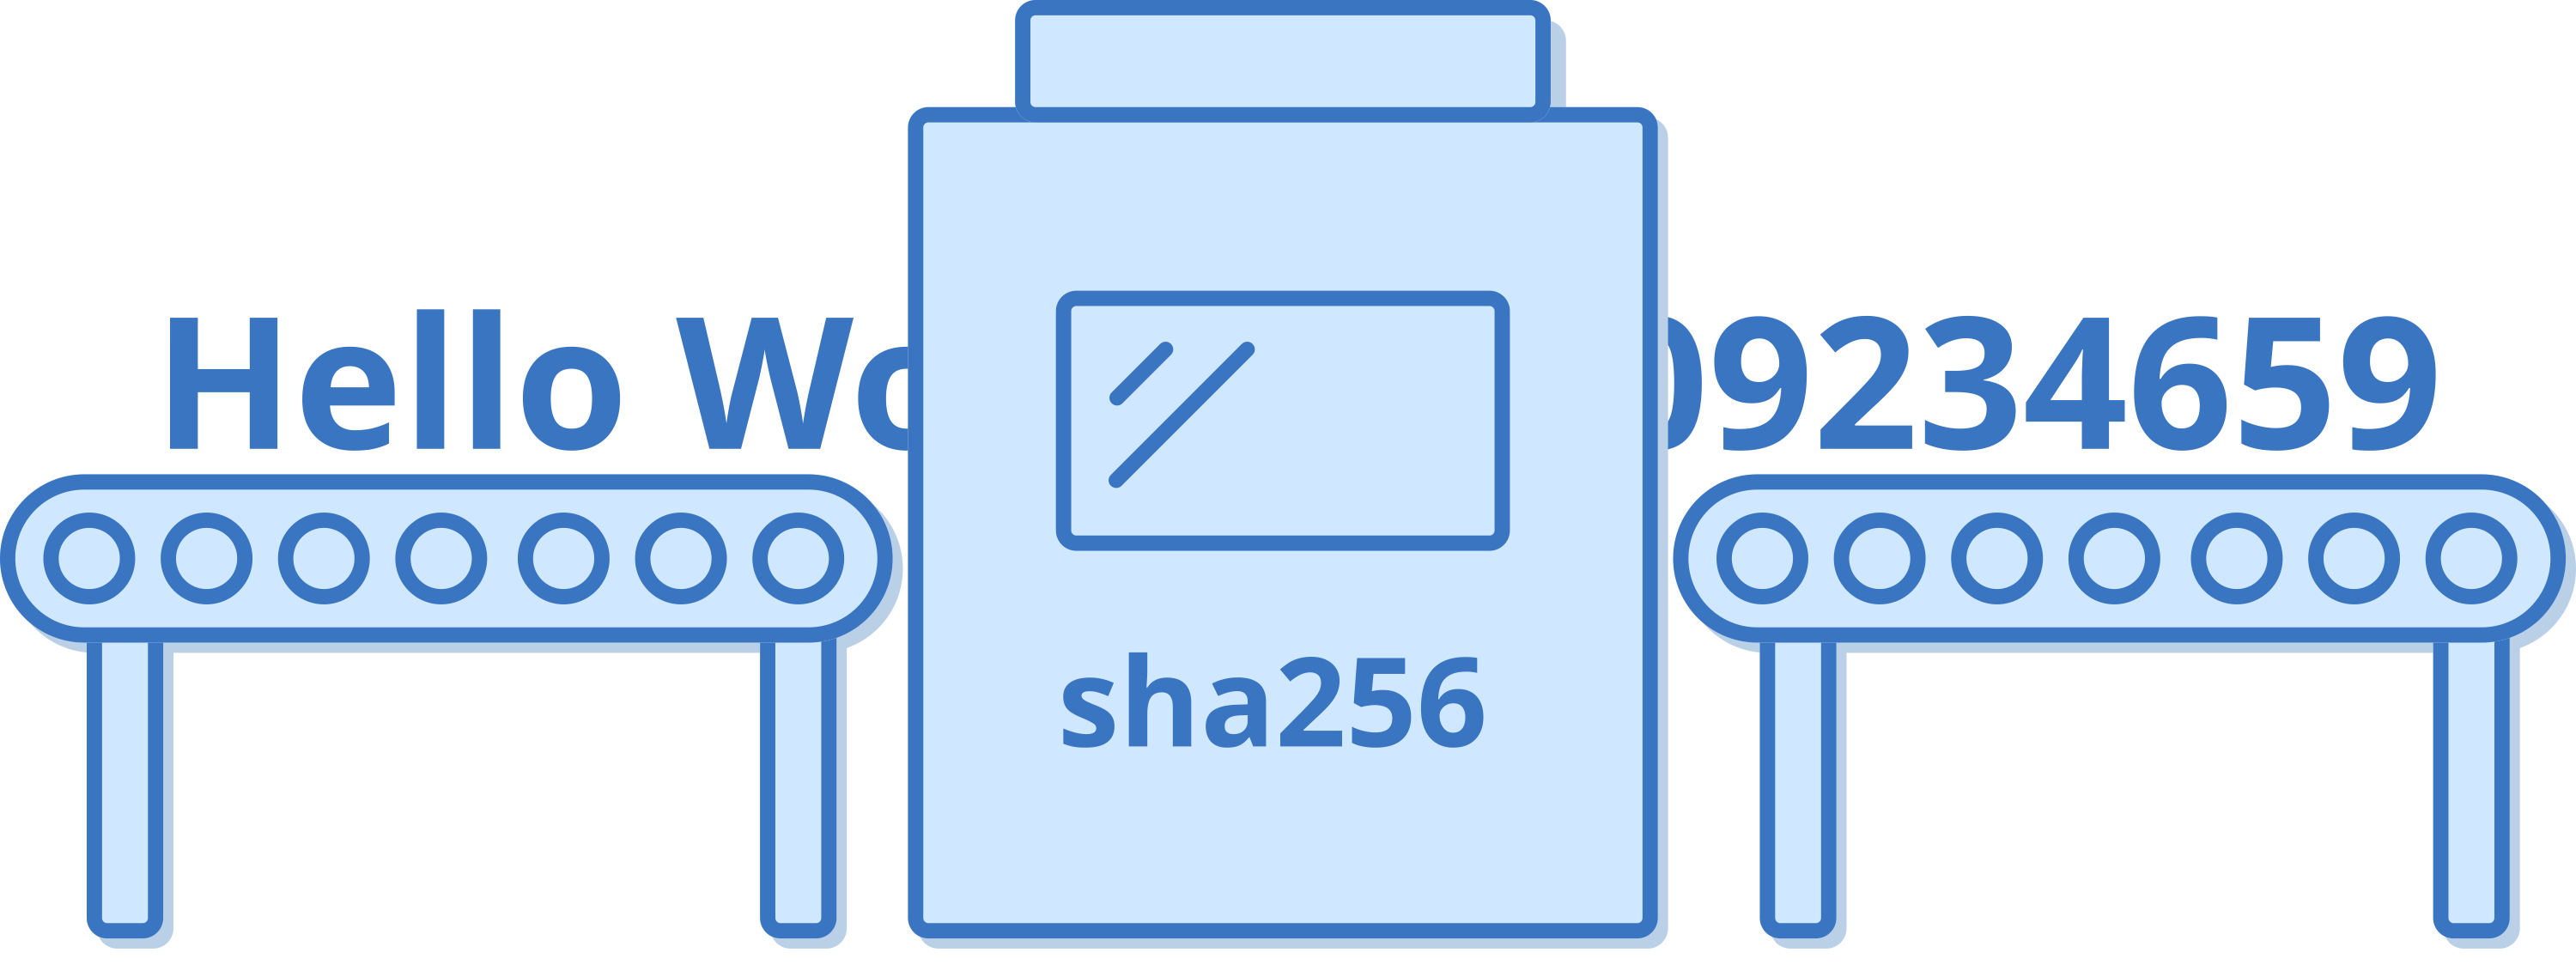
\includegraphics[width=\textwidth]{images/fig4.png}
    \caption{\footnotesize{\textit{Data gaat er aan de ene kant in, en aan de andere kant komt er een gigantisch onvoorspelbaar getal uit.}}}
    \label{fig4}
\end{figure}

\clearpage

De sha256 hash-functie bezit enkele eigenschappen die voor ons zeer nuttig zijn, namelijk:



\begin{enumerate}
    \item De uitkomst is deterministisch. Dat wil zeggen dat je bij dezelfde invoer altijd dezelfde uitvoer krijgt.
    \item De uitkomst is onvoorspelbaar. Indien slechts één letter van de invoer veranderd wordt, dan is de output \textit{volledig} anders, zonder enige correlatie met de oude invoer.
    \item De uitvoer-hash is snel te berekenen, onafhankelijk van de grootte van de invoer.
    \item Het is praktisch onmogelijk twee verschillende invoerwaardes te vinden die dezelfde uitvoer hebben.
    \item De sha256 functie is een eenrichtingsfunctie. Het is onmogelijk om de originele invoer te achterhalen vanuit de uitvoer.
    \item De uitvoer heeft altijd een specifieke grootte (256 \textit{bits} voor sha256).
\end{enumerate}

\section{Een korte uitleg over bits}

Het getallensysteem dat je gewend bent, bestaande uit de getallen 0 tot 9, staat bekend als het \textit{decimale} systeem omdat het tien cijfers telt. Computers hebben echter de voorkeur voor een ander getallenstelsel: een systeem dat is opgebouwd uit enen en nullen, die de aan- of afwezigheid van een elektrisch signaal aanduiden. Dit wordt het \textit{binaire} systeem genoemd.

In het decimale stelsel gebruik je slechts de cijfers $0$ tot en met $9$. Als je slechts één cijfer gebruikt, kun je tien verschillende getallen vertegenwoordigen, 0 tot en met 9. Als je twee cijfers gebruikt, kun je $10 \times 10 = 100$ verschillende getallen voorstellen: $00, 01,...$ tot en met $99$. Voor drie cijfers kun je $10 \times 10 \times 10 = 1000$ getallen hebben: $000, 001,...$ tot en met $999$.

Hopelijk begin je hier een patroon in te zien. Om erachter te komen hoe groot het getal is dat we kunnen voorstellen met N cijfers, vermenigvuldigen we tien, $N$ keer met zichzelf, oftewel $10^N$ ($10$ tot de macht van $N$).

Het binaire stelsel functioneert op dezelfde manier. Wat er verandert, is het aantal beschikbare cijfers. Terwijl we in het decimale stelsel gewend zijn aan tien cijfers, kan een \textit{binaire cijfer} of \textit{bit} slechts twee waarden aannemen: nul en één.

Als een \textit{bit} 2 waarden kan vertegenwoordigen, dan kunnen twee \textit{bits} 4 waarden vertegenwoordigen: $00, 01, 10, 11$. Je kunt dit berekenen door $2 \times 2$ te vermenigvuldigen, aangezien elk cijfer twee waarden kan hebben. Drie bits kunnen $2 \times 2 \times 2 = 2^3 = 8$ waarden vertegenwoordigen:  $000, 001, 010, 011, 100, 101, 110, 111$.

Een \textit{binair} getal dat N \textit{bits} lang is, kan dus $2^N$ verschillende waarden vertegenwoordigen.

Daarom is het aantal unieke waarden die je kunt vertegenwoordigen met 256 bits, de grootte van de sha256 hashing functie, $2^{256}$. Dat is een gigantisch, bijna onvoorstelbaar groot aantal. Weergegeven in decimaal, is getal dit 78 cijfers lang. Ter vergelijking is dit ongeveer dezelfde ordegrootte als het geschatte aantal atomen in het bekende universum.

  \vspace{\baselineskip}
$2^{256}$ = 115 792 089 237 316 195 423 570 985 008 687 907 853 269 984 665 640 564 039 457 584 007 913 129 639 936
\vspace{\baselineskip} 

Het bovenstaande getal representeert het aantal mogelijke uitkomsten van een sha256 hash-functie. Het is vrijwel onmogelijk om te voorspellen welk getal deze functie zal genereren. Dit zou vergelijkbaar zijn met het perfect voorspellen van de uitkomst van 256 opeenvolgende muntworpen, of het raden van de positie van een willekeurig atoom ergens in het universum.

Natuurlijk is dit getal te lang om steeds voluit te schrijven, dus we houden het vanaf nu simpelweg op $2^{256}$, maar ik hoop dat dit het ongelofelijke aantal mogelijkheden duidelijk heeft gemaakt.


\section{Laten we een aantal teksten gaan hashen}

Hier zijn enkele voorbeeldteksten en hun bijbehorende sha256 hashes. De output wordt getoond in decimale vorm, maar binnen in een computer zou dit de vertrouwde reeks van enen en nullen zijn.

Het gaat erom te laten zien hoe drastisch de output verandert op basis van slechts een kleine aanpassing aan de input, en aan te tonen dat je simpelweg niet kunt voorspellen wat de hash-functie zal genereren, ongeacht wat je erin invoert.

\begin{verbatim}
    “Hello World!”
    869913660443924676617831651669733090238
    07181648024718778313526389892860994842
   
    “Hello World!!”
    849402277206958989554476271088404243643
    90283616735576803008868844073193772558
    \end{verbatim}

Op basis van deze getallen is het voor niemand mogelijk om te achterhalen of te berekenen wat de initiële invoer was, zelfs niet voor een computer. Als je zelf eens wilt experimenteren met sha256, dan kun je dat proberen op \href{https://passwordsgenerator.net/sha256-hash-generator}{https://passwordsgenerator.net/sha256-hash-generator}.

\section{Hashen om de proof-of-work loterij te winnen}

Nu zijn we klaar om te praten over het belangrijkste stukje magie. We zeiden dat er $2^{256}$ totale mogelijke sha256-uitkomsten zijn. Voor de eenvoud van dit voorbeeld, laten we echter even aannemen dat er slechts 1000 verschillende resultaten mogelijk zijn.

Het loterijsysteem functioneert op de volgende manier:

\begin{enumerate}
    \item Alice kondigt aan dat ze 2 dollar naar \mbox{Bob} wil sturen.
    \item Iedereen die meespeelt, neemt de transactie \textquotedbl{}Alice geeft \$2 aan Bob\textquotedbl{}, en voegt hier een willekeurig getal aan toe, wat we een \textit{nonce} noemen.\footnote{Staat voor \textquotedbl{}number used only once\textquotedbl{}} Het gebruik van deze nonce zorgt ervoor dat hun input voor de sha256-hashfunctie verschilt van die van anderen, wat helpt bij het vinden van een winnend getal.
    \item Als dat getal kleiner is dan het \textit{doelnummer} (dit bespreken we verder in het volgende hoofdstuk), winnen ze de loterij.
    \item Als het getal dat ze krijgen groter is dan het doelnummer, dan hashen ze opnieuw, maar voegen dit keer een andere nonce toe: \textit{\textquotedbl{}Alice geeft \$2 aan Bob nonce=12345\textquotedbl{}}, dan \textit{\textquotedbl{}Alice geeft \$2 aan Bob nonce=92435\textquotedbl{}}, dan \textit{\textquotedbl{}Alice geeft \$2 aan Bob nonce=132849012348092134\textquotedbl{}}, enzovoort. Ze doen dit net zolang tot iemand een hash heeft gevonden die kleiner is dan het doelnummer.
 \end{enumerate}   
 
Het kan vele, vele pogingen kosten om een hash te vinden die kleiner is dan het doelnummer. We kunnen in feite bepalen hoe vaak iemand de loterij kan winnen door de kans dat ze een winnend getal vinden te manipuleren. Als er 1000 mogelijke hashes zijn, en we stellen het doelnummer in op 100, welk percentage van hashes zit er dan onder de doelnummer?

Dit is uiteraard vrij elementaire wiskunde; 100 van de 1000 mogelijkheden, oftewel 100/1000 = 10\% van de hashes zullen kleiner zijn dan het doelgetal. Dus als je een stuk tekst versleutelt en je hash-functie levert 1000 verschillende resultaten op, zou je verwachten dat 10\% van de hashes lager uitvallen dan het streefgetal van 100.

Dit werkt dus precies zo met onze loterij: we bepalen eerst een doelnummer. Vervolgens nemen we alle transacties die mensen aan het grootboek willen toevoegen en hashen deze met een willekeurig getal, de zogenaamde \textit{nonce}. Zodra iemand een hash vindt die onder het doelnummer valt, communiceert hij dit met het hele netwerk.

\begin{itemize}
    \item Ik heb de transacties \textquotedbl{}Alice stuurt \$2 naar Bob\textquotedbl{} en \textquotedbl{}Charlotte stuurt \$5 naar Alice\textquotedbl{} genomen.
    \item Ik heb hier de nonce \textquotedbl{}32895\textquotedbl{} aan toegevoegd. 
    \item De hash hiervan kwam uit op 42, wat minder is dan het afgesproken doelnummer van 100.
    \item Hier is mijn proof-of-work: de transactiegegevens, de nonce die ik heb gebruikt, en de hash die werd geproduceerd op basis van die inputs.
\end{itemize}

Het heeft mij misschien miljarden hash-pogingen en duizenden dollars aan energie gekost om deze hash te vinden, maar iedereen kan onmiddellijk valideren dat ik dit werk daadwerkelijk heb gedaan. Omdat ik zowel de invoergegevens (transacties en nonce) als de voorspelde uitkomst (het hash-getal) heb gedeeld, kan men dezelfde hash uitvoeren om in één keer te controleren of de gegevens die ik hen gegeven heb kloppen.

Hoe verhoudt dit zich tot energieverbruik? We gaven al eerder aan dat de verzameling van alle mogelijke hashes in feite een gigantisch getal is, vrijwel even groot als het aantal atomen in het universum. We kunnen het doelnummer zo laag instellen dat slechts een minuscule fractie van de hashes geldig is. Dit impliceert dat iedereen die een geldige hash wil vinden, zeer veel computertijd, en daarmee ook elektriciteit, zal moeten verbruiken om een hash te ontdekken die kleiner is dan ons doelnummer.

Hoe lager het doelnummer , hoe meer pogingen we nodig hebben om een geldig nummer te vinden en hoe hoger het doelnummer , des te sneller kunnen we een winnende hash vinden. Als onze kans om het juiste nummer te vinden een op een miljoen is, dan bewijst het vinden van dit nummer dat we ongeveer een miljoen berekeningen hebben gemaakt.

\begin{figure}[h]
    \centering
    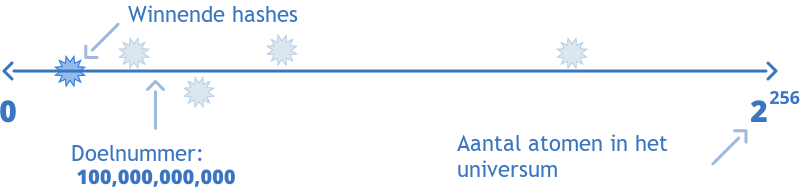
\includegraphics[width=\textwidth]{images/fig5.png}
    \caption{\footnotesize{\textit{We kunnen hashing zien als het rollen van een gigantische dobbelsteen op basis van specifieke invoergegevens, met een aantal zijden gelijk aan het aantal atomen in het universum. Alleen die invoergegevens die ervoor zorgen dat je onder het doelnummer rolt, winnen de loterij. Om de loterij te winnen, moet je aan de rest van het netwerk laten zien welke gegevens je hebt gebruikt om tot de uitkomst te komen.}}}
    \label{fig5}
\end{figure}
